%
%===============>>  ГРУППА 11-1 МОДУЛЬ 6  <<=============
%
\setmodule{6}

%BEGIN_FOLD % ====>>_____ Занятие 1 _____<<====
\begin{class}[number=1]
	\begin{listofex}
		\item Площадь грани прямоугольного параллелепипеда равна \( 15 \). Ребро, перпендикулярное этой грани, равно \(3\). Найдите объем параллелепипеда.
		\item Три ребра прямоугольного параллелепипеда, выходящие из одной вершины, равны \(4, 6, 9\). Найдите ребро равновеликого ему куба.
		\item Два ребра прямоугольного параллелепипеда, выходящие из одной вершины, равны \(3\) и \(4\). Площадь поверхности этого параллелепипеда равна \(94\). Найдите третье ребро, выходящее из той же вершины.
		\item Объем прямоугольного параллелепипеда равен \(24\). Одно из его ребер равно \(3\). Найдите площадь грани параллелепипеда, перпендикулярной этому ребру.
		\item Прямоугольный параллелепипед описан около сферы радиуса \(1\). Найдите его площадь поверхности.
		\item Диагональ куба равна \( 2\sqrt{3} \). Найдите объем куба и площадь его поверхности.
		\item Объем первого куба в \( 8 \) раз больше объема второго куба. Во сколько раз площадь поверхности первого куба больше площади поверхности второго куба?
		\item Найдите площадь боковой поверхности правильной шестиугольной призмы, сторона основания которой равна \( 5 \), а высота  --- \( 10 \).
		\item Дан куб \( ABCDA_1B_1C_1D_1 \). Площадь четырехугольника \( ABC_1D_1 \) равна \( 4\sqrt{2} \). Найдите площадь поверхности куба.
		\item 
		\begin{minipage}[t]{\bodywidth}
			В правильной треугольной пирамиде \(SABC\) с вершиной \(S\) биссектрисы треугольника \(ABC\) пересекаются в точке \(O\). Площадь треугольника \(ABC\) равна \(2\); объем пирамиды равен \(6\). Найдите длину отрезка \(OS\).
		\end{minipage}
		\hspace{0.02\linewidth}
		\begin{minipage}[t]{\picwidth}
			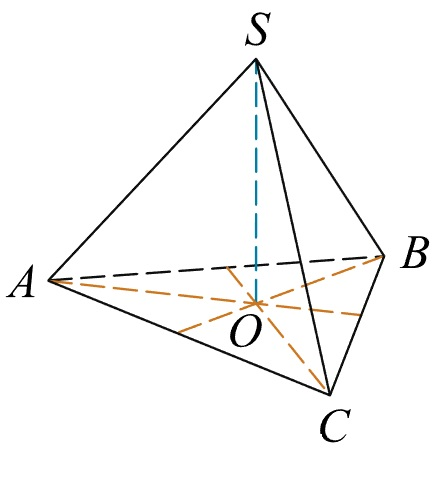
\includegraphics[align=t, width=\linewidth]{\picpath/G111M6L1-1}
		\end{minipage}
		\item В правильной четырехугольной пирамиде \(SABCD\) точка \(O\) --- центр основания, \(S\) --- вершина, \(SO=15, BD=16\). Найдите боковое ребро \(SA\).
		
		\item 
		\begin{minipage}[t]{\bodywidth}
			В правильной треугольной пирамиде \(SABC\) точка \(M\) --- середина ребра \(AB\), \(S\) --- вершина. Известно, что \(BC = 3\), а площадь боковой поверхности пирамиды равна \(45\). Найдите длину отрезка \(SM\).
		\end{minipage}
		\hspace{0.02\linewidth}
		\begin{minipage}[t]{\picwidth}
			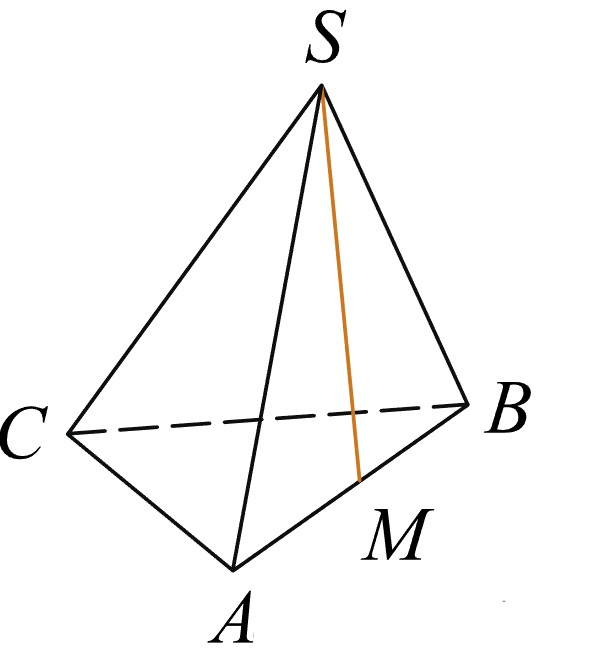
\includegraphics[align=t, width=\linewidth]{\picpath/G111M6L1-2}
		\end{minipage}
		\item Объем параллелепипеда \(ABCDA_1B_1C_1D_1\) равен \(9\). Найдите объем треугольной пирамиды \(ABCA_1\).
		\item Во сколько раз увеличится объем правильного тетраэдра, если все его ребра увеличить в два раза?
		\item В треугольнике \(ABC\) \(AB = 10, AC = BC\), высота \(AH = 8\). Найдите \(\cos{BAC}\).
		\item В треугольнике со сторонами \(9\) и \(6\) проведены высоты к этим сторонам. Высота, проведённая к первой из этих сторон, равна \(4\). Чему равна высота, проведённая ко второй стороне?
		\item Площадь параллелограмма \(ABCD\) равна \(24\). Точка \(M\) --- середина стороны \(BC\). Найдите площадь трапеции \(AMCD\).
	\end{listofex}
\end{class}
%END_FOLD

%BEGIN_FOLD % ====>>_____ Занятие 2 _____<<====
\begin{class}[number=2]
	\begin{listofex}
		\item 
		\begin{minipage}[t]{\bodywidth}
			На рисунке изображен многогранник, все двугранные углы многогранника прямые. Найдите квадрат расстояния между вершинами \(B_2\) и \(D_3\) .
		\end{minipage}
		\hspace{0.02\linewidth}
		\begin{minipage}[t]{\picwidth}
			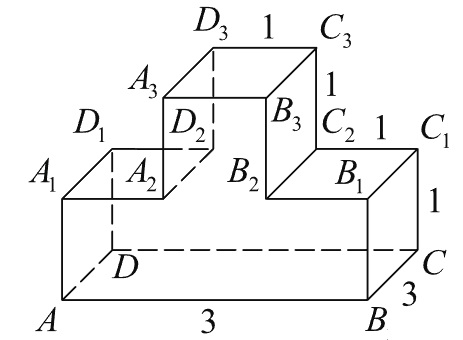
\includegraphics[align=t, width=\linewidth]{\picpath/G101M5L6-2}
		\end{minipage}
		\item С помощью этого же рисунка найдите:
		\begin{tasks}(1)
			\task расстояние между вершинами \(B\) и \(D_2\),
			\task тангенс угла \(C_2C_3B_2\).
		\end{tasks}
		\item 
		\begin{minipage}[t]{\bodywidth}
			На рисунке изображен многогранник, все двугранные углы многогранника прямые. Найдите его объём и площадь поверхности.
		\end{minipage}
		\hspace{0.02\linewidth}
		\begin{minipage}[t]{\picwidth}
			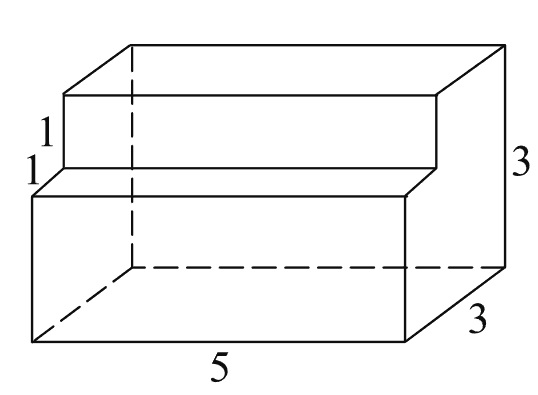
\includegraphics[align=t, width=\linewidth]{\picpath/G101M5L7-2}
		\end{minipage}
		\item 
		\begin{minipage}[t]{\bodywidth}
			На рисунке изображен многогранник, все двугранные углы многогранника прямые. Найдите его объём и площадь поверхности.
		\end{minipage}
		\hspace{0.02\linewidth}
		\begin{minipage}[t]{\picwidth}
			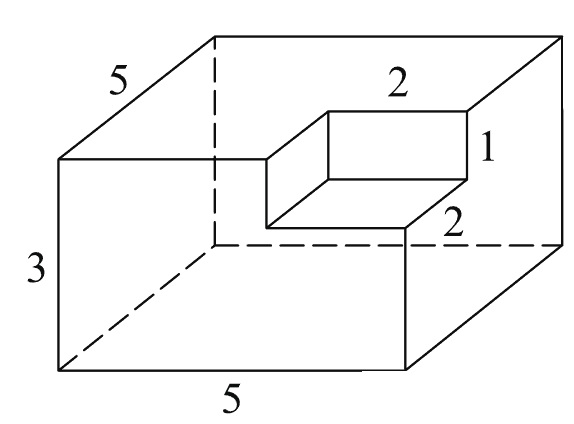
\includegraphics[align=t, width=\linewidth]{\picpath/G101M5L7-3}
		\end{minipage}
		\item 
		\begin{minipage}[t]{\bodywidth}
			На рисунке изображен многогранник, все двугранные углы многогранника прямые. Найдите его объём и площадь поверхности.
		\end{minipage}
		\hspace{0.02\linewidth}
		\begin{minipage}[t]{\picwidth}
			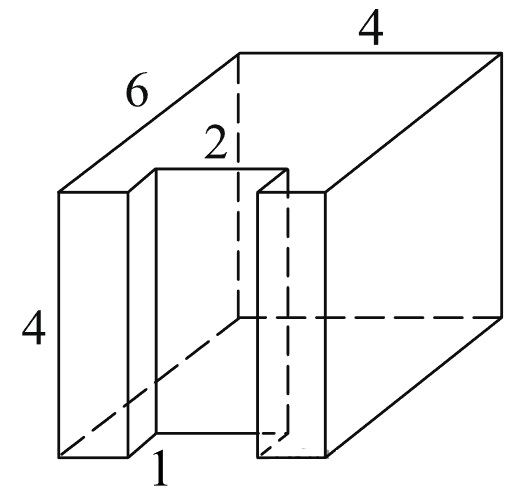
\includegraphics[align=t, width=\linewidth]{\picpath/G102M5L7-2}
		\end{minipage}
		\item 
		\begin{minipage}[t]{\bodywidth}
			На рисунке изображен многогранник, все двугранные углы многогранника прямые. Найдите его объём и площадь поверхности.
		\end{minipage}
		\hspace{0.02\linewidth}
		\begin{minipage}[t]{\picwidth}
			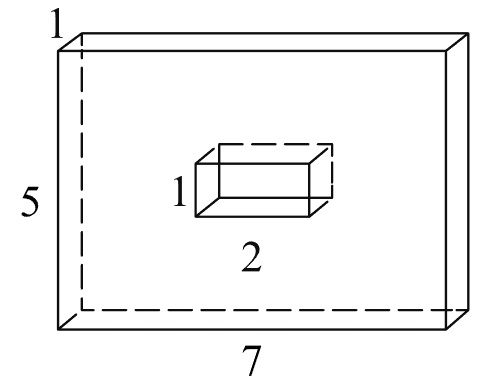
\includegraphics[align=t, width=\linewidth]{\picpath/G102M5L7-3}
		\end{minipage}
		\item 
		\begin{minipage}[t]{\bodywidth}
			На рисунке изображён многогранник, все двугранные углы многогранника прямые. Найдите расстояние между вершинами \(A\) и \(C_2\) .
		\end{minipage}
		\hspace{0.02\linewidth}
		\begin{minipage}[t]{\picwidth}
			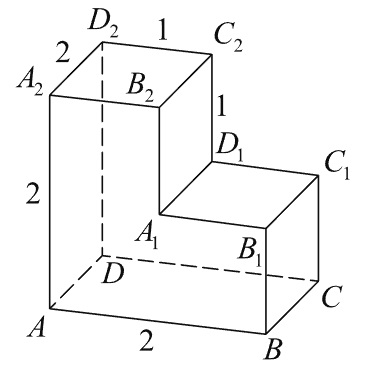
\includegraphics[align=t, width=\linewidth]{\picpath/G101M5L6-1}
		\end{minipage}
		\item С помощью этого же рисунка найдите расстояние между вершинами:
		\begin{tasks}(3)
			\task \(D\) и \(C_2\),
			\task \(B_1\) и \(D_2\),
			\task \(D_2\) и \(A_1\).
		\end{tasks}
		\item С помощью этого же рисунка найдите:
		\begin{tasks}(2)
			\task угол \( CAD_2 \),
			\task угол \( ABD \),
			\task тангенс угла \( B_2A_2C_2 \).
		\end{tasks}
	\end{listofex}
\end{class}
%END_FOLD

%BEGIN_FOLD % ====>>_ Домашняя работа 1 _<<====
\begin{homework}[number=1]
	\begin{listofex}
		\item Два ребра прямоугольного параллелепипеда, выходящие из одной вершины, равны \( 1 \), \( 2 \). Площадь поверхности параллелепипеда равна \( 16 \). Найдите его диагональ.
		\item Площадь грани прямоугольного параллелепипеда равна \( 12 \). Ребро, перпендикулярное этой грани, равно 4. Найдите объем параллелепипеда.
		\item Диагональ куба равна \( 4 \). Найдите площадь его поверхности.
		\item Ребра прямоугольного параллелепипеда равны \( 7 \), \( 12 \) и \( 5 \). Найдите объем и площадь поверхности этого параллелепипеда.
		\item В правильной треугольной пирамиде \(SABC\) медианы основания \(ABC\) пересекаются в точке \(O\). Площадь треугольника \(ABC\) равна \(9\); объем пирамиды равен \(6\). Найдите длину отрезка \(OS\).
		\item В правильной треугольной пирамиде \(SABC\) медианы основания \(ABC\) пересекаются в точке \(O\). Площадь треугольника \(ABC\) равна \(2\); объем пирамиды равен \(5\). Найдите длину отрезка \(OS\).
		\item В правильной четырехугольной пирамиде \(SABCD\) точка \(O\) --- центр основания, \(S\) --- вершина, \(SB=13, AC=24\). Найдите длину отрезка \(SO\).
		\item В правильной четырехугольной пирамиде \(SABCD\) точка \(O\) --- центр основания, \(S\) --- вершина, \(SO=8, BD=30\). Найдите боковое ребро \(SC\).
		\item Основанием пирамиды является прямоугольник со сторонами \(3\) и \(4\). Ее объем равен \(16\). Найдите высоту этой пирамиды.
		\item Стороны основания правильной шестиугольной пирамиды равны \(10\), боковые ребра равны \(13\). Найдите площадь боковой поверхности этой пирамиды.
	\end{listofex}
\end{homework}
%END_FOLD

%BEGIN_FOLD % ====>>_____ Занятие 3 _____<<====
\begin{class}[number=3]
	\begin{listofex}
		\item Занятие 3 
	\end{listofex}
\end{class}
%END_FOLD

%BEGIN_FOLD % ====>>_____ Занятие 4 _____<<====
\begin{class}[number=4]
	\begin{listofex}
		\item Занятие 4
	\end{listofex}
\end{class}
%END_FOLD

%BEGIN_FOLD % ====>>_ Домашняя работа 2 _<<====
\begin{homework}[number=2]
	\begin{listofex}
		\item Домашняя работа 2
	\end{listofex}
\end{homework}
%END_FOLD

%BEGIN_FOLD % ====>>_____ Занятие 5 _____<<====
\begin{class}[number=5]
	\begin{listofex}
		\item Занятие 5
	\end{listofex}
\end{class}
%END_FOLD
	
%BEGIN_FOLD % ====>>_____ Занятие 6 _____<<====
\begin{class}[number=6]
	\begin{listofex}
		\item Занятие 6
	\end{listofex}
\end{class}
%END_FOLD
	
%BEGIN_FOLD % ====>>_ Домашняя работа 3 _<<====
\begin{homework}[number=3]
	\begin{listofex}
		\item Домашняя работа 3
	\end{listofex}
\end{homework}
%END_FOLD

%BEGIN_FOLD % ====>>_____ Занятие 7 _____<<====
\begin{class}[number=7]
	\title{Подготовка к проверочной}
	\begin{listofex}
		\item Занятие 7
	\end{listofex}
\end{class}
%END_FOLD

%BEGIN_FOLD % ====>>_ Проверочная работа _<<====
\begin{exam}
	\begin{listofex}
		\item Проверочная
	\end{listofex}
\end{exam}
%END_FOLD